\documentclass[oneside,openany,headings=optiontotoc,11pt,numbers=noenddot]{article}

\usepackage[a4paper]{geometry}
\usepackage[utf8]{inputenc}
\usepackage[T1]{fontenc}
\usepackage{lmodern}
\usepackage[ngerman]{babel}
\usepackage{ngerman}

\usepackage[onehalfspacing]{setspace}

\usepackage{fancyhdr}
\usepackage{fancybox}

\usepackage{rotating}
\usepackage{varwidth}

%Struktogramme
\usepackage[german,curves]{struktex}

\usepackage{pdflscape}
\usepackage{changepage}
\usepackage{graphicx}
\usepackage[bottom]{footmisc}
\usepackage{transparent}
\usepackage{graphbox}
\graphicspath{
	{Pics/PDFs/}
	{Pics/JPGs/}
	{Pics/PNGs/}
}
\usepackage{caption}
\usepackage{wrapfig}
\usepackage{marginnote}
\usepackage{tabularx}
\usepackage{dashrule}
\usepackage{soulutf8}
\usepackage{hhline}
%arydshln suppresses vertical lines in table
%\usepackage{arydshln}
\usepackage{multirow}
\usepackage{enumerate}
\usepackage[hidelinks]{hyperref}
\usepackage{listings}

\usepackage[table]{xcolor}
\usepackage{array}
\usepackage{enumitem,amssymb,amsmath}
\usepackage{interval}
\usepackage{cancel}
\usepackage{stmaryrd}
\usepackage{wasysym}
\usepackage{polynom}
\usepackage{diagbox}
\usepackage{dashrule}
\usepackage{framed}
\usepackage{mdframed}
\usepackage{karnaugh-map}
\usepackage{pdfpages}

\usepackage{blindtext}

\usepackage{eso-pic}

\usepackage{amssymb}
\usepackage{eurosym}

\usepackage[pages=some]{background}
\pagestyle{headings}
\renewcommand{\headrulewidth}{0.2pt}
\renewcommand{\footrulewidth}{0.2pt}
\newcommand*{\underdownarrow}[2]{\ensuremath{\underset{\overset{\Big\downarrow}{#2}}{#1}}}
\setlength{\fboxsep}{5pt}
\newcommand{\explainBelow}[3]{\underbrace{#1}_{\parbox{\widthof{#3}}{\footnotesize\raggedright #2}}}
\newcommand{\explainAbove}[3]{\overbrace{#1}^{\parbox{\widthof{#3}}{\footnotesize\raggedright #2}}}
\newcommand\footnoteref[1]{\protected@xdef\@thefnmark{\ref{#1}}\@footnotemark}


% Codestyle defined
\definecolor{codegreen}{rgb}{0,0.6,0}
\definecolor{codegray}{rgb}{0.5,0.5,0.5}
\definecolor{codepurple}{rgb}{0.58,0,0.82}
\definecolor{backcolour}{rgb}{0.95,0.95,0.92}
\definecolor{deepgreen}{rgb}{0,0.5,0}
\definecolor{darkblue}{rgb}{0,0,0.65}
\definecolor{mauve}{rgb}{0.40, 0.19,0.28}
\colorlet{exceptioncolour}{yellow!50!red}
\colorlet{commandcolour}{blue!60!black}
\colorlet{numpycolour}{blue!60!green}
\colorlet{specmethodcolour}{violet}

%Neue Spaltendefinition
\newcolumntype{L}[1]{>{\raggedright\let\newline\\\arraybackslash\hspace{0pt}}m{#1}}
\newcolumntype{M}{>{\centering\arraybackslash}X}
\newcommand{\cmnt}[1]{\ignorespaces}
%Textausrichtung ändern
\newcommand\tabrotate[1]{\rotatebox{90}{\raggedright#1\hspace{\tabcolsep}}}

%Intervall-Konfig
\intervalconfig {
	soft open fences
}

%Bash
\lstdefinestyle{BashInputStyle}{
	language=bash,
	basicstyle=\small\sffamily,
	backgroundcolor=\color{backcolour},
	columns=fullflexible,
	backgroundcolor=\color{backcolour},
	breaklines=true,
}
%Java
\lstdefinestyle{JavaInputStyle}{
	language=Java,
	backgroundcolor=\color{backcolour},
	aboveskip=1mm,
	belowskip=1mm,
	showstringspaces=false,
	columns=flexible,
	basicstyle={\footnotesize\ttfamily},
	numberstyle={\tiny},
	numbers=none,
	keywordstyle=\color{purple},,
	commentstyle=\color{deepgreen},
	stringstyle=\color{blue},
	emph={out},
	emphstyle=\color{darkblue},
	emph={[2]rand},
	emphstyle=[2]\color{specmethodcolour},
	breaklines=true,
	breakatwhitespace=true,
	tabsize=2,
}
%Python
\lstdefinestyle{PythonInputStyle}{
	language=Python,
	alsoletter={1234567890},
	aboveskip=1ex,
	basicstyle=\footnotesize,
	breaklines=true,
	breakatwhitespace= true,
	backgroundcolor=\color{backcolour},
	commentstyle=\color{red},
	otherkeywords={\ , \}, \{, \&,\|},
	emph={and,break,class,continue,def,yield,del,elif,else,%
		except,exec,finally,for,from,global,if,import,in,%
		lambda,not,or,pass,print,raise,return,try,while,assert},
	emphstyle=\color{exceptioncolour},
	emph={[2]True,False,None,min},
	emphstyle=[2]\color{specmethodcolour},
	emph={[3]object,type,isinstance,copy,deepcopy,zip,enumerate,reversed,list,len,dict,tuple,xrange,append,execfile,real,imag,reduce,str,repr},
	emphstyle=[3]\color{commandcolour},
	emph={[4]ode, fsolve, sqrt, exp, sin, cos, arccos, pi,  array, norm, solve, dot, arange, , isscalar, max, sum, flatten, shape, reshape, find, any, all, abs, plot, linspace, legend, quad, polyval,polyfit, hstack, concatenate,vstack,column_stack,empty,zeros,ones,rand,vander,grid,pcolor,eig,eigs,eigvals,svd,qr,tan,det,logspace,roll,mean,cumsum,cumprod,diff,vectorize,lstsq,cla,eye,xlabel,ylabel,squeeze},
	emphstyle=[4]\color{numpycolour},
	emph={[5]__init__,__add__,__mul__,__div__,__sub__,__call__,__getitem__,__setitem__,__eq__,__ne__,__nonzero__,__rmul__,__radd__,__repr__,__str__,__get__,__truediv__,__pow__,__name__,__future__,__all__},
	emphstyle=[5]\color{specmethodcolour},
	emph={[6]assert,range,yield},
	emphstyle=[6]\color{specmethodcolour}\bfseries,
	emph={[7]Exception,NameError,IndexError,SyntaxError,TypeError,ValueError,OverflowError,ZeroDivisionError,KeyboardInterrupt},
	emphstyle=[7]\color{specmethodcolour}\bfseries,
	emph={[8]taster,send,sendMail,capture,check,noMsg,go,move,switch,humTem,ventilate,buzz},
	emphstyle=[8]\color{blue},
	keywordstyle=\color{blue}\bfseries,
	rulecolor=\color{black!40},
	showstringspaces=false,
	stringstyle=\color{deepgreen}
}

\lstset{literate=%
	{Ö}{{\"O}}1
	{Ä}{{\"A}}1
	{Ü}{{\"U}}1
	{ß}{{\ss}}1
	{ü}{{\"u}}1
	{ä}{{\"a}}1
	{ö}{{\"o}}1
}

% Neue Klassenarbeits-Umgebung
\newenvironment{worksheet}[3]
% Begin-Bereich
{
	\newpage
	\sffamily
	\setcounter{page}{1}
	\ClearShipoutPicture
	\AddToShipoutPicture{
		\put(55,761){{
				\mbox{\parbox{385\unitlength}{\tiny \color{codegray}BBS I Mainz, #1 \newline #2
						\newline #3
					}
				}
			}
		}
		\put(455,761){{
				\mbox{\hspace{0.3cm}
\includegraphics[width=0.2\textwidth]{../../logo.pdf}}
			}
		}
	}
}
% End-Bereich
{
	\clearpage
	\ClearShipoutPicture
}

\pagestyle{plain}

\geometry{left=1.50cm,right=1.50cm,top=2.50cm,bottom=1.00cm,includeheadfoot}

\begin{document}
	\begin{worksheet}{BS EGSIE 18}{1. Lehrjahr, LF 4 - Informationstechnische Systeme bereitstellen}{Verarbeitungsgeräte - Intern}
		\onehalfspacing
		\clearpage
		\setcounter{page}{7}
		\setcounter{section}{1}
		\setcounter{subsection}{2}
		\subsection{Chipsatz und Bussysteme}
		\subsubsection*{Bestandteile des Chipsatzes}
		Als \glqq{}Chipsatz\grqq{} bezeichnet man alle Bausteine auf dem Mainboard. Zusammen erfüllen diese zahlreiche Steuerungsaufgaben und sind für eine reibungslose Zusammenarbeit aller Komponenten zuständig. Hauptbestandteile sind:
		\begin{itemize}[label=-]
			\item integrierte Grafikeinheit bzw Grafikanbindung über PEG\footnote{PCI Express for Graphics} oder AGB (veraltet)
			\item Speicher-Controller
			\item PCI-Express-Controller
			\item PCI-/PCI-X-Controller
			\item Controller für Laufwerke\footnote{EIDE/ATA, SATA/eSATA, SAS/SCSI, Diskette.}
			\item Controller für externe Schnittstellen (z.B. USB, FireWire, Thunderbolt)
			\item Legacy-Schnittstelle: PS/2, parallel, seriell (alle veraltet)
		\end{itemize}
		Üblicherweise bestand der Chipsatz aus zwei Chips:\\
		\par\noindent
		\begin{minipage}[l]{0.48\textwidth}
			\begin{itemize}[label=-]
				\item Northbridge, bei Intel oft als \textbf{MCH} (Memory Controller Hub) bezeichnet (1). Ist zuständig für die schnelle Anbindung des Hauptspeichers und der Grafik an die CPU (2).
				\item Southbridge, bei Intel auch \textbf{IHC} (I/O-Controller Hub) (3). Fasst alle Verbindungen zusammen, die nicht zeitkritisch sind (z.B. Sound, LAN, USB etc.)
			\end{itemize}
			Die Bezeichnungen North-/Southbridge entstanden durch die typishcen Positionen der Chips auf dem Mainboard.
		\end{minipage}
		\hfill
		\begin{minipage}[c]{0.48\textwidth}
			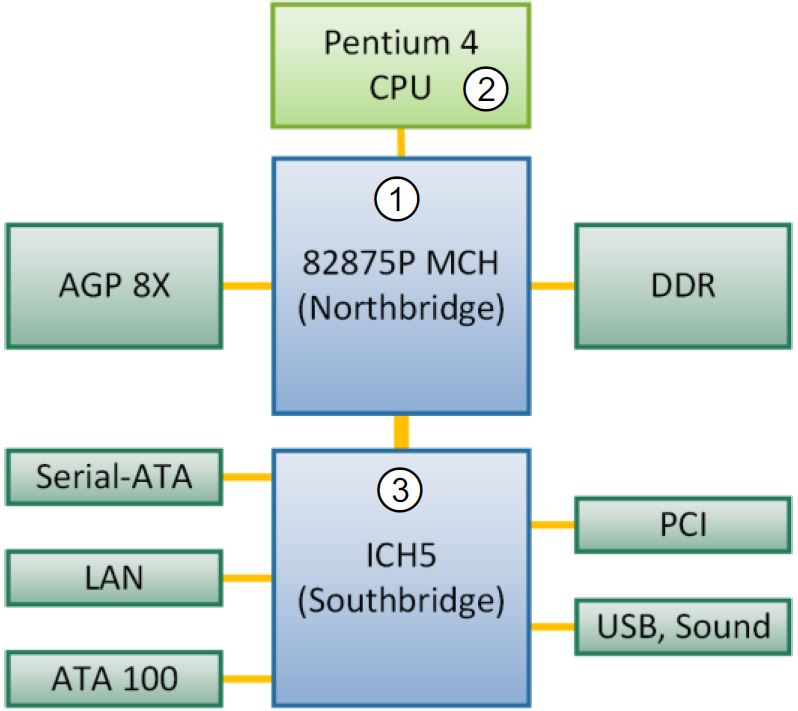
\includegraphics[width=0.8\textwidth]{../99_Bilder/ChP4.jpg}
		\end{minipage}\\
		\par\noindent
		AMD integrierte ab der K8-Serie den Speichercontroller der Northbridge in den Prozessor.\\
		\par\noindent
		\begin{minipage}[l]{0.48\textwidth}
			Auch Intel integrierte in der Core-i7-Serie den Speichercontroller in den Prozessor.\\
			Bei neueren Modellreihen\footnote{Ab 2011.} ist auch die Anbindung der Grafikkarte über PCIe bzw. der Grafikkern selbst im Prozessor verbaut. Somit sind alle Funktionen der Northbridge in den Prozessor gewandert (1).\\
			Die übrigen Funktionen können somit in einem Chip zusammengefasst werden.
		\end{minipage}
		\hfill
		\begin{minipage}[c]{0.48\textwidth}
			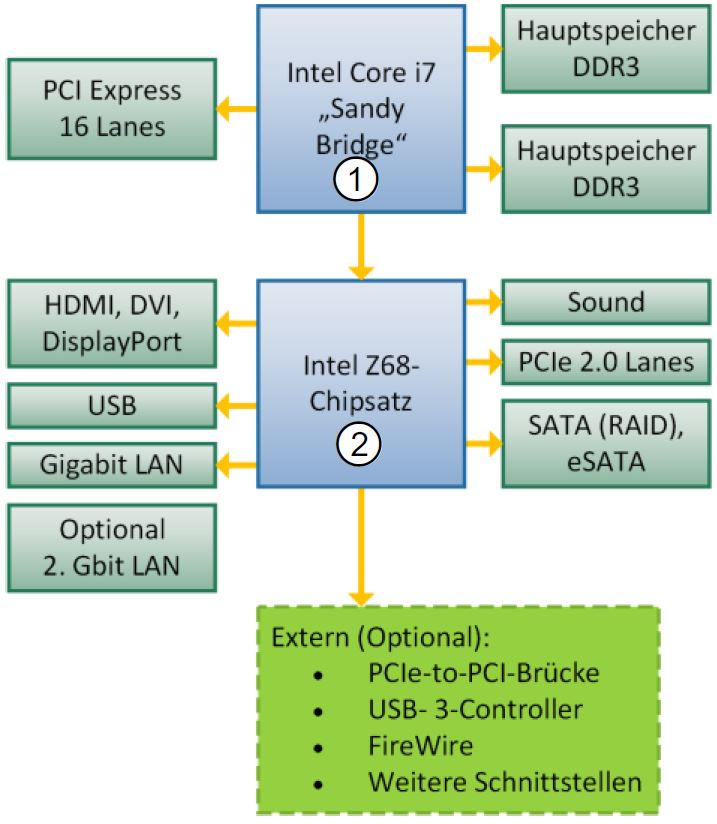
\includegraphics[width=0.8\textwidth]{../99_Bilder/Chi7.jpg}
		\end{minipage}
		\subsubsection*{BIOS-Chip}
		\footnotesize{}Eigentlich ist der BIOS-Chip kein \textit{richtiger} Bestandteil des Mainboards. Dennoch ließe sich kein PC ohne ebendiesen Chip starten.\normalsize\\
		\par\noindent
		Im BIOS-Chip befinden sich alle Programmroutinen, de zum Starten des Computers und zum Erkennen und Ansprechen der verwendeten Hardware nötig sind.\\
		Die Software, die sich auf diesem Chip befindet, kann bei Bedarf durch eine neuere Software-Version ersetzt werden. Diesen Vorgang bezeichnet man weitläufig als BIOS-Update oder auch als \glqq{}Flashen\grqq{} des BIOS.\\
		Das BIOS an sich existiert bereits seit ungefähr 30 Jahren. Da viele Hersteller ihre eigenen BIOS-Varianten nutzen, herrscht ein entsprechendes \glqq{}Wirrwarr\grqq{}.\\		
		\par\noindent
		Entsprechend wurde um 2000 von Intel eine Initiative zum \glqq{}BIOS-Ersatz\grqq{} gestartet. In Zusammenschluss mit anderen Prozessor-, PC- und BIOS-Herstellern wurde die \textbf{Unified EFI} ins Leben gerufen.\\
		Ziele der EFI sind u.a.:
		\begin{itemize}[label=-]
			\item einfachere Bedienung 	als beim herkömmlichen BIOS
			\item aktuelle Hardware unterstützen
			\item Fernwartungsmöglichkeiten implementieren
			\item hohe Auflösungen aktueller Grafikkarten vor dem Start des Betriebssystems nutzen können
			\item vorgeschaltete Bootloader überflüssig machen
		\end{itemize}
		Kritiker bemängeln bei EFI-Boards die sicherheits- und datenschutztechnischen Problematiken.\\
		Dennoch ist ein EFI ab einer Systemplattengröße von 2 TB zwingend erforderlich.
		\subsubsection*{Das Bussystem}
		Ein \textbf{Bussystem} verbindet verschiedene Komponenten\footnote{Prozessor, Controller, Arbeitsspeicher, Eingabe-/Ausgabeports.} des PC elektrisch miteinander. Auf diese Weise kann ein Austausch von Informationen stattfinden.\\
		Ein Bussystem ist so als Bündel elektrischer Leitungen realisiert, dass die betreffenden Baugruppen in Parallelschaltung angeschlossen sind.\\
		\par\noindent
		Möchte man ein \underline{schnelles} Bussystem verwenden, greift man auf den \textbf{Host-Bus} oder \textbf{Front Side Bus} (FSB) zurück. Diese ermöglichen eine Kommunikation zwischen der CPU und der Northbridge und den dort angeschlossenen Komponenten RAM und Grafikkarte.\\
		Zusätzlich ermöglicht die Northbridge auch die Verbindung zur Southbridge. Diese verfügt über \textbf{I/O-Bussysteme} für weitere Peripheriegeräte.
		\subsubsection*{I/O-Bussysteme}
		Häufig werden Peripheriegeräte über Steckplätze (Slots) für Erweiterungskarten\footnote{interne Schnittstellen.} mit dem Computer verbunden. Für die Kommunikation mit diesen Erweiterungskarten existieren verschiedene I/O-Bussystem.\\
		Aktuell werden folgende I/O-Bussysteme verbaut:
		\begin{itemize}
			\item PCIe (Peripheral Component Interconnect Express) für moderne Grafikkarten
			\item S-ATA (Serial Advanced Technology Attachment) für Festplatten und optische Laufwerke (BD-/DVD-/CD-R/W)
		\end{itemize}
		In älteren Geräten finden sich auch noch AGP\footnote{Accelerate Graphics Port.}, PCI, EIDE/IDE-Bus und CNR.
		\newpage
		\subsection{Die Funktion der CPU}
		Im PC werden die wesentlichen Teile in einem zentralen Baustein zusammengefasst, der \textbf{Central Processing Unit} (CPU oder auch Prozessor).\\
		Die CPU kontrolliert den Datenfluss zwischen den einzelnen Funktionseinheiten. Dabei entstammen die Daten dem Arbeitsspeicher oder den angeschlossenen Geräten (Tastatur, Laufwerk etc). Nachdem die übermittelten Daten verarbeitet wurden, wird das Ergebnis an den Arbeitsspeicher oder an ein angeschlossenes Gerät weitergeleitet.\\
		Die CPU lädt dabei eigenständig den nächsten Befehl zur Datenverarbeitung nach. Die eigentliche Aufgabe der CPU besteht dann im Berechnen und Verschieben der Daten.
		\begin{framed}
			\noindent\footnotesize
			\textbf{Exkurs}: Bei dem in \textit{1.2 Datenverarbeitung im PC} erwähnten Von-Neumann-Rechner werden die Befehle und Daten sequenziell\footnote{Also schrittweise nacheinander.} aus dem Speicher abgearbeitet. Das heißt, dass das Bussystem sich als Flaschenhals bzw. Engpass entpuppt, da vor und nach jedem Verarbeitungsschritt dieselbe Leitung verwendet wird.\\
			\par\noindent
			Eine Verbesserung konnte mit einer hierarchisch gegliederten Speicherstruktur erreicht werden. Diese Speicherstruktur besteht aus Registern und verschiedenen Speicherebenen (Cache-Ebenen).\\
			Daten die häufig verwendet werden können so in separaten schnellen Cache-Speichern abgelegt werden. Zudem ist mit modernen CPU-Generationen, durch die feinere Aufteilung der Funktionseinheiten und der Erweiterung der Befehlssätze, eine teilweise parallele Arbeitsweise erreicht werden.
		\end{framed}
		\normalsize
		\subsubsection*{Steuerwerk / Leitwerk}
		Das Steuerwerk ist die mitunter umfangreichste Zusammenfassung unterschiedlicher Funktionsblöcke. Es besteht aus den verschiedenen Kontrolleinheiten, in denen sämtliche Vorgänge im Computer kontrolliert und gesteuert werden.
		\subsubsection*{Befehlsdecoder}
		Der Befehlsdecoder (IDU - Instruction Decode Unit) ist auf dem Prozessor oft mehrmals in einer parallelen Anordnung vorhanden. Dies erlaubt eine kürzere Zeitspanne für die Befehlsdurchführung. Auch die Ausführungseinheit (EXU - Execution Unit) ist bei vielen Prozessoren mehrmals vorhanden.
		\subsubsection*{Rechenwerk}
		Zum Rechenwerk gehören neben der ALU (Arithmetic Logic Unit) und der FPU (Floating Point Unit) auch Register, in denen Daten zwischengespeichert werden können. Nur mithilfe der ALU kann der Prozessor Gleichheits- und Ungleichheitsprüfungen sowie Größenbestimmungen durchführen. Nur dann können alle Anweisungen eines Programms abgearbeitet werden.
		\subsubsection{Leistungsmerkmale der CPU}
		Die wichtigsten Eigenschaften von Prozessoren lassen sich am einfachsten mit folgenden Kenngrößen und Technologien beschreiben:
		\begin{itemize}[label=-]
			\item Taktfrequenz (intern und extern)
			\item Anzahl der pro Sekunde verarbeiteten Befehle (MIPS)
			\item Anzahl der pro Sekunde verarbeiteten Gleitkomma-Operationen (FLOPS)
			\item Art des Befehlssatzes oder die Möglichkeiten zur parallelen Abarbeitung von Befehlen (multithreading)
			\item Zahl der CPU-Kerne im Prozessorgehäuse (Multi-Core-Prozessoren)
			\item Cache
			\item Busbreite (64-Bit)
			\item Art des Befehlssatzes (CISC, RISC)
		\end{itemize}
		Dabei ist der \textbf{C}omplex \textbf{I}nstruction \textbf{S}et \textbf{C}omputer (CISC) der am bekanntesten. Sie verfügen über sehr leistungsfähige, aber auch sehr komplexe Befehlssätze. Mit diesen können mithilfe eines einzelnen Befehls umfangreiche Operationen ausgeführt werden.\\
		Beim \textbf{R}educed \textbf{I}nstruction \textbf{S}et \textbf{C}omputer hingegen, werden einfachere Befehlssätze verwendet, so dass schnellere Ausführzeiten erreicht werden. Diese besitzen zwar nur einen eingeschränkten Befehlssatz, können diese aber meist vollständig in einem Taktzyklus ausführen.\\
		Um umfangreichere Befehle verarbeiten zu können, werden diese in mehrere einfachere Teile zerlegt und nacheinander ausgeführt.
		\subsubsection*{Taktfrequenz / CPU-Geschwindigkeit}
		Daten und Befehle werden in einem festgelegten Rhythmus verarbeitet. Dieser Rhythmus wird durch einen Taktgeber (clock) vorgegeben. Die Anzahl der Taktimpulse pro Sekunde entspricht physikalisch einer Frequenz und hat die Einheit \textbf{Hertz} (1 Megahetz = 1MHz = 1 Millionen Taktimpulse pro Sekunde).\\
		\par\noindent
		Ein Befehl, der von der CPU ausgeführt wird, benötigt eine bestimmte Anzahl von Taktimpulsen. Das bedeutet, je höher die Taktfrequenz ist, umso schneller können einzelne Programmanweisungen bearbeitet werden.
		\begin{framed}
			\noindent
			Ein Programm, das von einer CPU mit 1 GHz in 30 Sekunden ausgeführt wird, kann von einer vergleichbaren 2 GHz CPU in 15 Sekunden verarbeitet werden.
		\end{framed}
		\noindent
		Zum Vergleich von CPUs einer Familie eines Herstellers kann die Taktrate als Leistungsmerkmal herangezogen werden. Dennoch sollte beachtet werden, dass eine höhere Taktfrequenz nicht automatisch auch eine höhere Leistung bedeutet. Interessanter ist die Betrachtung der Anzahl der parallel verarbeitbaren Befehle pro Taktzyklus.\\
	\end{worksheet}
\end{document}